\cotefile{143}

\scanpage{8}
\mspage{4}
une application
\[
(22)\qquad\widetilde{\mathfrak X}'(i)\xrightarrow{\Phi_i}\operatorname{Hom}(\mathbf T(\overline{\mathbf Q}),\pi_1(\mathfrak X'))
\]
\margin{ici il faut supposer $\dim\mathfrak X=1$ -- autrement il
faut \unsure{voir|revoir} la définition de $\widetilde{\mathfrak X}'(I)$.....\\
autre façon de dire -- il faut que $\widetilde{\mathfrak X}'$ \unsure{soit considéré}
\unsure{pour donner des|pour définir des} \unsure{traits} \unsure{henséliens ou locaux au}
dessus d'un pt de $\unsure{\overline{\mathfrak X}'(I)|\mathfrak X'(I)}$\unsure{.....|....}}
compatible avec les opérations de $\pi_1(\mathfrak X')$
de part et d'autre, et qui précise
la donnée de $\unsure{\varphi|\varphi_i}$ (17). Mieux encore,
le système $(\Phi_i)_{i\in I}=\Phi$.
\[
(23)\qquad\widetilde{\mathfrak X}'(I)\xrightarrow{\Phi}\operatorname{Hom}(\mathbf T(\overline{\mathbf Q}),\pi_1(\mathfrak X'))
\]
est compatible avec les $\unsure{\mathcal E|\Sigma}_{\mathfrak X'}\deleted{\unsure{\mathcal E}}$ de part et
d'autre, en se rappelant, pour l'opération
de $\unsure{\mathcal E|\Sigma}_{\mathfrak X'}$ sur le mb de droite, de tenir
compte aussi de l'opération de $\unsure{\mathcal E|\Sigma}_{\mathfrak X'}$
sur $\mathbf T(\overline{\mathbf Q})$ (via $\Gamma$).

\textcircled{5} Soit enfin, par dessus le marché, une
partie $J\subset\mathfrak X'(\overline{\mathbf Q})$. Soit $\widetilde{\mathfrak X}'(J)$ son
image inverse dans $\widetilde{\mathfrak X}'$. Soit $\mathcal G_{\mathfrak X'}(I,J)$
ou simplement $\mathcal G'$ le sous-groupe de $\mathcal G_{\mathfrak X'}(I)$
qui invarie $J$. \deleted{D. Voici les structures} \inserted{Donc $\mathcal G'$}
opère sur $J$, sur $\widetilde{\mathfrak X}'(J)$ et sur
\[
(24)\qquad\widetilde{\mathfrak X}'(J)\longrightarrow J
\]
\mspage{7}

\scanpage{9}
Enfin, on a une famille de scindages \inserted{partiels}
\[
(25)\qquad\Psi^{\deleted{\unsure{\mathrm{ext}}}}=(\Psi_j)_{j\in J}:\bigl(\widetilde{\mathfrak X}'(j)\longrightarrow\operatorname{Hom}(\mathcal G'_j,\unsure{\mathcal E'|\Sigma'}_{\deleted{\mathfrak X'}})\bigr)
\]
(où cette fois $\unsure{\mathcal E'|\Sigma'}$ désigne l'image inverse
de $\mathcal G'\subset\mathcal G_{\mathfrak X'}$ dans $\unsure{\mathcal E|\Sigma}_{\mathfrak X'}$, 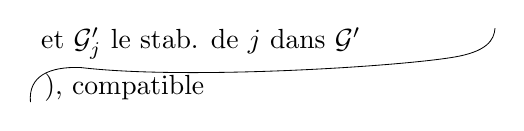
\begin{tikzpicture}[baseline=(base.base)]
\node[anchor=base west,inner sep=0] (base) at (0,0) {), compatible};
\node[anchor=base west,inner sep=0] at (-.04,.58) {\inserted{et $\mathcal G'_j$ le stab. de $j$ dans $\mathcal G'$}};
\draw[line width=.3pt] (-.17,-.10) .. controls (-.20,.24) and (.08,.35) .. (.46,.34) .. controls (1.80,.18) and (4.48,.35) .. (5.20,.47) .. controls (5.63,.54) and (5.72,.69) .. (5.73,.84);
\end{tikzpicture}
avec les opérations de $\unsure{\mathcal E'|\Sigma'}$ de part et
d'autre, \deleted{s'inscrivant dans une famille de
scindages mod op. de $\pi_1$}
\[
\deleted{(26)\qquad\Psi^{\mathrm{ext}}=(\Psi_j^{\mathrm{ext}})_{j\in J}:\bigl(\widetilde{\mathfrak X}'(J)\unsure{\bigr)}\longrightarrow\operatorname{Hom}(\unsure{\mathcal G'|\mathcal G'_j},\unsure{\mathcal E'|\Sigma'})/\operatorname{Int}(\pi_1,\unsure{\mathcal E'|\Sigma'})}
\]
\deleted{également compatible avec op. de $\unsure{\mathcal E'|\Sigma'}$\unsure{.}}

\textcircled{6} \uuline{Récapitulons.} On a donc : \deleted{$\mathfrak X$
schéma de t.f. sur $\overline{\mathbf Q}$, un divi}
\[
\mathrm I\quad\left\{\begin{array}{l}
\mathfrak X\text{ de t.f. sur }\overline{\mathbf Q}\\
D=\sum_{i\in I}D_i\text{ diviseur effectif sur }\mathfrak X\text{ à comp.}\\
\qquad\text{simples, }\mathfrak X\text{ lisse en les pts maximaux}\\
\qquad\text{de }\operatorname{supp}D\\
J\underset{\text{\unsure{\uline{fini}}}}{\subset}\mathfrak X'(\overline{\mathbf Q}),\quad\text{où }\mathfrak X'=\mathfrak X-D
\end{array}\right.
\]
On pose\margin{(}
\[
\mathrm{II}\quad\left\{\begin{array}{l}
\mathcal G'=\text{gr des autom du schéma \inserted{absolu} }\mathfrak X\\
\qquad\text{qui invarie }D\text{ et }J\\
G'=\text{ss-gp de }\mathcal G'\text{ formé des }\overline{\mathbf Q}\text{-autom.}\\
\mathbf T(\overline{\mathbf Q})=\varprojlim_n\mu_n(\overline{\mathbf Q})\\[1ex]
\Gamma=\operatorname{Gal}(\overline{\mathbf Q}/\mathbf Q)
\end{array}\right.
\]
\mspage{8}

\scanpage{10}
\mspage{5}
d'où
\[
(1)\qquad1\longrightarrow G'\longrightarrow\mathcal G'\longrightarrow\Gamma
\]
et un germe de relèvement
\[
(2)\qquad\diagram{\begin{tikzcd}[ampersand replacement=\&]
\mathcal G'\arrow[r]\&\Gamma\arrow[d,phantom,"\cup" description,"{\text{ss-gp ouvert}}"']\\
\&\Gamma'\arrow[ul]
\end{tikzcd}}
\]
\margin{pour mémoire : relation avec variations des corps de base\ldots}
\uline{Choisissons} (cf normalisations plus bas)
\textcircled{$\overline{\underline{\mathrm{III}}}$} \uline{un rev. universel}
$\widetilde{\mathfrak X}'$ de $\mathfrak X'$,
d'où
\deleted{posons}
\[
\pi_1(\mathfrak X')=\operatorname{Aut}(\widetilde{\mathfrak X}'/\mathfrak X')
\]
On trouve alors

(3) \deleted{(3)} structure d'extension
\[
1\longrightarrow\pi_1(\mathfrak X')\longrightarrow\unsure{\mathcal E|\Sigma}'\longrightarrow\mathcal G'\mathbin{-}1
\]
\margin{pour mémoire : relation entre p\textsuperscript{ts} de $\mathfrak X'(\overline{\mathbf Q})$ et scindages partiels de l'extension (3)\ldots}
\[
(4)\qquad\unsure{\mathcal E|\Sigma}'\text{-ensembles}\quad\left\{\begin{array}{l}\widetilde{\mathfrak X}'(I)\\\widetilde{\mathfrak X}'(J)\end{array}\right.
\]
(5) Opérations de $\unsure{\mathcal E|\Sigma}'$ sur $I,J$ via $\mathcal G'$, et
$\unsure{\mathcal E|\Sigma}'$-applications
\[
\left\{\begin{array}{l}
\widetilde{\mathfrak X}'(\unsure{\Delta|I})\mathbin{-}I\\
\widetilde{\mathfrak X}'(J)\mathbin{-}J\simeq\widetilde{\mathfrak X}'(J)/\pi_1
\end{array}\right.
\]
\mspage{9}

\scanpage{12}
\mspage{\unsure{6}}
Programme du \deleted{paradigme \unsure{de théorie des|de la théorie des}} \inserted{``gruppentheoretisches} Gleichnis'' (paradigme en termes de théorie des groupes) de l'\inserted{arithmétique :}\deleted{\unsure{arithm.} géométrie algébrique absolue (en car. 0).}

a) Donner une description ``gruppentheoretisch'' complète de $\Gamma$

b) Donner une description complète de tous les éléments de structure énumérés ci-dessus, dans des cas typiques importants pour $(\mathfrak X,D,J)$, dont nous indiquons quelques-uns plus bas.

\margin{On tâchera de prendre $\mathfrak X$ propre autant que possible (quitte à compléter\ldots)}

\uline{NB} Quand on a les éléments de structure envisagés pour $(\mathfrak X,D,J)$, on les a aussi automatiquement pour \unsure{tt|$\forall$} 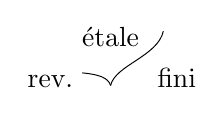
\begin{tikzpicture}[baseline=(rev012.base)]
\node[anchor=base west,inner sep=0pt] (rev012) at (0,0) {rev.};
\node[anchor=base west,inner sep=0pt] at (1.65,0) {fini};
\node[anchor=base,inner sep=0pt] at (1.06,.52) {\inserted{étale}};
\draw[line width=.35pt] (.70,.19) .. controls (.91,.17) and (1.03,.13) .. (1.06,.03);
\draw[line width=.35pt] (1.06,.03) .. controls (1.12,.29) and (1.66,.40) .. (1.73,.72);
\end{tikzpicture} de $\mathfrak X'....$ Il faudrait expliciter ce point avec soin, et expliciter également dans les $=$ optiques les foncteurs ``bouchage de trous'' (en rajoutant 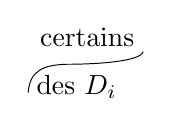
\begin{tikzpicture}[baseline=(des012.base)]
\node[anchor=base west,inner sep=0pt] (des012) at (.12,0) {des $D_i$};
\node[anchor=base,inner sep=0pt] at (.77,.61) {\inserted{certains}};
\draw[line width=.35pt] (.02,.02) .. controls (.04,.31) and (.23,.37) .. (.50,.38)
  .. controls (.93,.38) and (1.45,.42) .. (1.48,.54);
\end{tikzpicture} qu'on avait enlevés) ou ``forage des trous'' 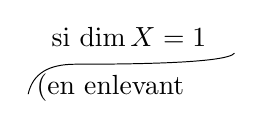
\begin{tikzpicture}[baseline=(en012.base)]
\node[anchor=base west,inner sep=0pt] (en012) at (.12,0) {(en enlevant};
\node[anchor=base,inner sep=0pt] at (1.30,.61) {\inserted{si $\dim\mathfrak X=1$}};
\draw[line width=.35pt] (.02,.01) .. controls (.08,.28) and (.29,.39) .. (.62,.39)
  .. controls (1.28,.39) and (2.54,.40) .. (2.64,.53);
\end{tikzpicture} certains des $\xi\in J$).
\mspage{11}

\scanpage{14}
\mspage{7}
En fait, si $Y'\longleftrightarrow E$, on a
\[
\begin{aligned}
Y'(I)&\simeq\widetilde{\mathfrak X}'(I)\mathbin{\wedge}_{\pi_1}E\\
Y'(J)&\simeq\widetilde{\mathfrak X}'(J)\mathbin{\wedge}_{\pi_1}E
\end{aligned}
\]
et les \deleted{\unsure{appl.}} isomorphismes (11) reviennent à des iso.
\[
\left\{\begin{aligned}
\widetilde{\mathfrak X}'(I)\mathbin{\wedge}_{\pi_1}E&\simeq(\widetilde{\mathfrak X}'(I)\mathbin{\wedge}_{\pi_1}B_\gamma)\mathbin{\wedge}_{\pi_1}E\\
\widetilde{\mathfrak X}'(J)\mathbin{\wedge}_{\pi_1}E&\simeq(\widetilde{\mathfrak X}'(J)\mathbin{\wedge}_{\pi_1}(B_\gamma))\mathbin{\wedge}_{\pi_1}E
\end{aligned}\right.
\]
qu'on peut décrire à l'aide d'isom. de $\pi_1$-ens à droite
\[
\left\{\begin{aligned}
\widetilde{\mathfrak X}'(I)&\simeq\widetilde{\mathfrak X}'(I)\mathbin{\wedge}_{\pi_1}B_\gamma\\
\widetilde{\mathfrak X}'(J)&\simeq\widetilde{\mathfrak X}'(J)\mathbin{\wedge}_{\pi_1}B_\gamma
\end{aligned}\right.
\]
lesquels reviennent à la donnée d'hom
\diagram{\(\left\{\begin{array}{l}
\begin{tikzcd}[ampersand replacement=\&]
B_\gamma \arrow[r,dash,"{\unsure{}}" description] \& {\unsure{\overline{\mathrm A}|\mathrm A}\mathrm{ut}}_{\deleted{\unsure{\mathrm{ens}}}}(\widetilde{\mathfrak X}'(I))=\operatorname{Bij}(\widetilde{\mathfrak X}'(I),\widetilde{\mathfrak X}'(I))
\end{tikzcd}\\
\text{et itou pour }\widetilde{\mathfrak X}'(J)
\end{array}\right.\)}
compatibles avec les op de $\pi_1$ à g. et à dr.
Or la donnée de ces applications, pour $\gamma\in\Gamma'$ variable, équivaut \deleted{\unsure{peut se}} à la donnée d'\deleted{une}applications
\diagram{\begin{tikzcd}[ampersand replacement=\&]
\unsure{\mathcal E'|\Sigma'}_{\Gamma'}=\displaystyle\bigcup_{\gamma\in\Gamma'}B_\gamma \arrow[r] \& \operatorname{Aut}_{\mathrm{ens}}(\widetilde{\mathfrak X}'(I))\\
{} \arrow[r] \& \operatorname{Aut}_{\mathrm{ens}}(\widetilde{\mathfrak X}'(J))
\end{tikzcd}}
et celle qu'on cherche est justement l'opération déduite par celles déjà envisagées de $\unsure{\mathcal E'|\Sigma'}$ sur $\widetilde{\mathfrak X}'(I)$, $\widetilde{\mathfrak X}'(J)\ldots.$
\mspage{13}

\scanpage{15}
\textcircled{7} Réconstruction des I-groupoïde fondamentaux $\Pi_1(\mathfrak X';J)$ de $\mathfrak X'$, et des opérations de $\mathcal G'$ dessus, en termes de l'extension $\unsure{\mathcal E|\Sigma}'$ de $\mathcal G'$ par $\pi_1$, et de l'opération de $\unsure{\mathcal E|\Sigma}'$ sur $\widetilde{\mathfrak X}'(J)$ et $\widetilde{\mathfrak X}'(J)\longrightarrow J$ [et des applications (7) (8)
\diagram{\begin{tikzcd}[ampersand replacement=\&]
\Psi^{\mathrm{ex}}:\widetilde{\mathfrak X}'(J) \arrow[r] \& \operatorname{Splitt}(\unsure{\mathcal E|\Sigma}'/\mathcal G')/\pi_1
\end{tikzcd}}
\diagram{\begin{tikzcd}[ampersand replacement=\&]
\Psi_{\unsure{j}}:\bigl(\widetilde{\mathfrak X}'(j) \arrow[r,dash] \& \operatorname{Splitt}(\unsure{\mathcal E|\Sigma}'_j/\mathcal G'_j)\bigr)].
\end{tikzcd}}
\margin{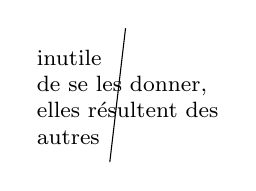
\begin{tikzpicture}[x=1cm,y=1cm]
\node[anchor=north west,align=left,font=\footnotesize] at (0,0) {inutile\\de se les donner,\\elles résultent des\\autres};
\draw (1.25,0.15) -- (1.05,-1.55);
\end{tikzpicture}}
\[
\operatorname{Ob}\Pi_1=J
\]
\deleted{\unsure{Soit} $j,j'\in J$}

\uline{NB} si $\widetilde\xi\in\widetilde{\mathfrak X}'(J)$, $\widetilde{\mathfrak X}'[j]$ (rev universel de $\mathfrak X'$ en $j$) s'identifie à $\widetilde{\mathfrak X}'$ (puisque $\widetilde\xi$ est un p\textsuperscript{t} marqué de $\widetilde{\mathfrak X}'$ au dessus de $j$
\diagram{\begin{tikzcd}[ampersand replacement=\&]
\widetilde{\mathfrak X}' \arrow[r,"\unsure{\varphi|\psi}_{\widetilde\xi}"] \& \widetilde{\mathfrak X}'[j]
\end{tikzcd}}
Si $\gamma\in\pi_1$, on aura
\[
\Psi_{\gamma\cdot\widetilde\xi}=\Psi_{\widetilde\xi}\circ\gamma_{\widetilde{\mathfrak X}'}^{\deleted{\unsure{-1}}}
\]
donc on peut dire, indépendamment du choix du p\textsuperscript{t} base $\widetilde\xi$
\diagram{\begin{tikzcd}[ampersand replacement=\&]
\widetilde{\mathfrak X}'[j] \& 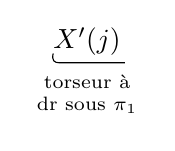
\begin{tikzpicture}[baseline=(torsorfactor.base),x=1cm,y=1cm]
\node[inner sep=0pt] (torsorfactor) at (0,0) {$\mathfrak X'(j)$};
\draw (-0.43,-0.15) .. controls (-0.45,-0.24) and (-0.42,-0.27) .. (-0.35,-0.27) -- (0.48,-0.27);
\node[anchor=north,align=center,font=\scriptsize] at (0,-0.30) {torseur à\\dr sous $\pi_1$};
\end{tikzpicture}\mathbin{\wedge}_{\pi_1}\widetilde{\mathfrak X}' \arrow[l,"\sim"']
\end{tikzcd}}
\mspage{14}

\scanpage{16}
\mspage{8}
Ceci noté, on aura donc, si $j,j'\in J=\operatorname{Ob}\Pi_1$
\[
\begin{aligned}
\operatorname{Isom}_{\Pi_{1,\unsure{\mathrm f|\phi}}}(j,j')&\overset{\mathrm{dfn}}{=}\operatorname{Isom}(\widetilde{\mathfrak X}'[j],\widetilde{\mathfrak X}'[j'])\\
&\simeq\operatorname{Isom}_{\pi_1\text{-tors à droite}}(\widetilde{\mathfrak X}'(j),\widetilde{\mathfrak X}'(j'))
\end{aligned}
\]
la composition des chemins étant la composition des hom de $\pi_1$-tors\unsure{.} à droite.
\deleted{\unsure{Comme}} On a donc reconstruit 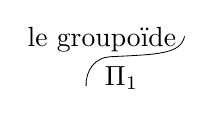
\begin{tikzpicture}[baseline=(object.base)]
\node[inner sep=0pt] (object) at (0,0) {$\Pi_1$};
\node[anchor=south,inner sep=0pt] at (-.25,.32) {\inserted{le groupoïde}};
\draw[line width=.3pt] (-.45,-.10) .. controls (-.46,.10) and (-.33,.26) .. (-.15,.27) .. controls (.45,.30) and (.75,.30) .. (.80,.53);
\end{tikzpicture} à l'aide de $\widetilde{\mathfrak X}'(J)$ et de l'opération libre (à droite) de $\pi_1$ sur $\widetilde{\mathfrak X}'(J)$.
\deleted{[les opérations} Comment reconstituer l'opération de $\mathcal G'$ sur $\Pi_1$ ? L'opération sur $\operatorname{Ob}\Pi_1=J$ n'est autre que l'opération donnée de $\mathcal G'$ sur $J$ (factorisant celle de $\unsure{\mathcal E'|\Sigma'}$). Soit $g\in\mathcal G'$, explicitons
\diagram{\begin{tikzcd}[ampersand replacement=\&]
\operatorname{Isom}_{\Pi_1}(j,j') \arrow[r,"{\substack{g_{\Pi_1}\\[-.3ex]\sim}}"] \arrow[d,equal] \& \operatorname{Isom}(gj,gj') \arrow[d,equal]\\
\operatorname{Isom}_{\pi_1}(\widetilde{\mathfrak X}'(j),\widetilde{\mathfrak X}'(j')) \arrow[r,"{\substack{?\\[-.3ex]\sim}}"] \& \operatorname{Isom}_{\pi_1}(\widetilde{\mathfrak X}'(gj),\widetilde{\mathfrak X}'(gj'))
\end{tikzcd}}
Pour ceci, considérons le 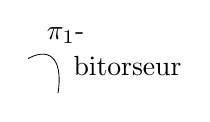
\begin{tikzpicture}[baseline=(word.base)]
\node[anchor=base west,inner sep=0pt] (word) at (0,0) {bitorseur};
\node[anchor=base east,inner sep=0pt] at (.15,.46) {\inserted{$\pi_1$-}};
\draw[line width=.3pt] (-.57,.22) .. controls (-.25,.39) and (-.13,.15) .. (-.19,-.22);
\end{tikzpicture}
\[
B_g\unsure{:}\subset\unsure{\mathcal E'|\Sigma'}\qquad\text{image inv. de }g\text{ par }\unsure{\mathcal E'|\Sigma'}\unsure{\mathbin{-}|\longrightarrow}\mathcal G'
\]
On note que l'on a (grâce à l'op. de $\unsure{\mathcal E'|\Sigma'}$ sur $\widetilde{\mathfrak X}'(I)$]
\[
\begin{aligned}
\widetilde{\mathfrak X}'(gj)&\simeq\widetilde{\mathfrak X}'(j)\mathbin{\wedge}_{\pi_1}B_g\\
\widetilde{\mathfrak X}'(gj')&\simeq\widetilde{\mathfrak X}'(j')\mathbin{\wedge}_{\pi_1}B_g
\end{aligned}
\]
\mspage{15}

\scanpage{17}
d'où aussitôt la flèche envisagée.

Il faudrait encore expliciter comment (7) (8) résultent de la donnée de l'opération de $\unsure{\mathcal E|\Sigma}'$ sur $\widetilde{\mathfrak X}'(J)$, induisant une opération \uline{libre} de $\pi_1\subset\unsure{\mathcal E|\Sigma}'$ sur $\widetilde{\mathfrak X}'(J)$ (ayant $J$ comme ens quotient)\ldots.

\uline{Reformulation}

Considérons les systèmes
\[
\left\{\begin{gathered}
\diagram{\begin{tikzcd}[ampersand replacement=\&]
1 \arrow[r,dash] \& \pi \arrow[r,dash] \& \unsure{\mathcal E|\Sigma} \arrow[r,dash] \& \mathcal G \arrow[r,dash] \& 1 \& \text{ext. de groupes}
\end{tikzcd}}\\
\mathfrak Z\quad\unsure{\mathcal E|\Sigma}\text{-ens }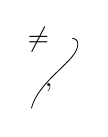
\begin{tikzpicture}[baseline=(comma.base)]
\node[anchor=base,inner sep=0pt] (comma) at (0,0) {$,$};
\node[anchor=base,inner sep=0pt] at (-.13,.50) {$\inserted{\ne\varnothing}$};
\draw[line width=.3pt] (-.22,-.28) .. controls (-.13,.06) and (.30,.29) .. (.36,.48) .. controls (.39,.58) and (.35,.60) .. (.30,.61);
\end{tikzpicture}\text{ où }\pi\subset\unsure{\mathcal E|\Sigma}\text{ opère librement}
\end{gathered}\right.
\]
Ils forment une \uline{catégorie} $C$

Considérons les systèmes $(\Pi,\widetilde\Pi,p,\mathcal G,g)$ où $\Pi$ est un groupoïde \begin{tikzpicture}[baseline=(word.base)]
\node[anchor=base west,inner sep=0pt] (word) at (0,0) {connexe};
\node[anchor=base east,inner sep=0pt] at (.20,.52) {\inserted{\unsure{\begin{tikzpicture}[baseline=-.35ex,x=.5cm,y=.5cm,line cap=round]
\draw[line width=.35pt] (.07,.49) .. controls (.16,.46) and (.27,.39) .. (.27,.28)
  .. controls (.27,.13) and (.08,.11) .. (.09,.24)
  .. controls (.10,.34) and (.20,.39) .. (.25,.32);
\draw[line width=.45pt] (.46,.36)--(.68,.34);
\end{tikzpicture}}}};
\draw[line width=.3pt] (-.18,-.20) .. controls (-.28,.02) and (-.02,.27) .. (.36,.42) .. controls (.51,.50) and (.53,.57) .. (.40,.60);
\end{tikzpicture}, $p:\widetilde\Pi\longrightarrow\Pi$ un rev. universel de $\Pi$, et $\mathcal G$ un groupe opérant \deleted{\unsure{sur|de}} sur $\Pi$ par automorphismes par $a:\mathcal G\longrightarrow\operatorname{Aut}(\Pi)$. Ils forment une catégorie $C'$. On va définir des équivalences quasi-inverses l'une de l'autre
\diagram{\begin{tikzcd}[ampersand replacement=\&]
C \arrow[r,shift left,"\alpha"] \& C' \arrow[l,shift left,"\beta"]
\end{tikzcd}}
\mspage{16}

\scanpage{18}
\mspage{9}
\uline{Définition de $\alpha$}\qquad On va définir
\[
\alpha(\unsure{\mathcal E|\Sigma},\mathcal G,\pi,\mathfrak Z\mathord{\begin{tikzpicture}[x=1ex,y=1ex,baseline=0pt]
\fill (0.10,0.23) circle (0.08);
\draw[line width=0.45pt,line cap=round] (0.39,0.18)--(0.71,0.18);
\end{tikzpicture}})=(\Pi,\widetilde\Pi,p,\mathcal G,a)
\]
\[
\left\{\begin{array}{l}
\operatorname{Ob}\Pi=\mathfrak Z/\pi\unsure{.}\quad(\text{soit }J)\\
\operatorname{Isom}(j,j')=\operatorname{Isom}_{\pi}(\mathfrak Z_j,\mathfrak Z_{j'})\\
\text{composition des flèches évidente}
\end{array}\right.\qquad\bigg|\quad\text{d'où groupoïde }\Pi
\]
\[
\deleted{\widetilde\Pi_j=\mathfrak Z_j}\qquad\operatorname{Ob}\widetilde\Pi=\mathfrak Z
\]
\diagram{\begin{tikzcd}[ampersand replacement=\&]
\operatorname{Isom}(z,z')=\{\mathrm{pt}\}\arrow[d]\&\begin{gathered}\forall z,z'\in\mathfrak Z\\(\widetilde\Pi\text{ cat. discrète}\mathord{\begin{tikzpicture}[x=1ex,y=1ex,baseline=0pt]
\fill (0.10,0.23) circle (0.08);
\draw[line width=0.45pt,line cap=round] (0.39,0.18)--(0.71,0.18);
\end{tikzpicture}})\end{gathered}\\
\operatorname{Isom}(j,j')\simeq\operatorname{Isom}(\mathfrak Z_j,\mathfrak Z_{j'})\&
\end{tikzcd}}
\deleted{(\unsure{où} $j,j'$ \unsure{les} \unsure{images}\unsure{)}}\inserted{(si $j=\dot z$, $j'=\dot z'$)}
\margin{\figure{\begin{tikzpicture}[x=1cm,y=1cm]
\draw (0,0.20)--(0,-2.40);
\node[anchor=west,inner sep=0pt] at (0.15,0) {$\widetilde\Pi$ cat. \uline{discrète}};
\node[anchor=west,inner sep=0pt] at (0.15,-0.38) {sur $\Pi$ définie par};
\node[anchor=west,inner sep=0pt] at (0.15,-0.86) {foncteur};
\node[anchor=west,inner sep=0pt] at (0.95,-0.60) {\inserted{\unsure{contr.}}};
\draw[thin] (0.94,-0.64) .. controls (0.75,-0.66) and (0.57,-0.74) .. (0.45,-0.83);
\node[inner sep=0pt] at (0,-1.35) {$\Longleftarrow$};
\node[anchor=west,inner sep=0pt] at (0.15,-1.45) {\begin{tikzcd}[ampersand replacement=\&,column sep=small]
F:\Pi^\circ\arrow[r]\&\operatorname{Ens}
\end{tikzcd}};
\node[anchor=west,inner sep=0pt] at (0.15,-2.10) {$F(j)=\mathfrak Z_j,\ldots$};
\node[anchor=west,inner sep=0pt] at (0.15,-2.72) {$\widetilde\Pi\simeq\Pi_{/F}$};
\end{tikzpicture}}}
$\downarrow$ transforme l'unique \unsure{pt|p\textsuperscript{t}} de $\operatorname{Isom}(z,z')$ en l'unique 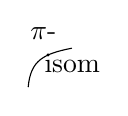
\begin{tikzpicture}[baseline=(iso.base),x=1cm,y=1cm]
\node[anchor=base west,inner sep=0pt] (iso) at (0,0) {isom};
\node[anchor=base west,inner sep=0pt] at (-0.18,0.42) {\inserted{$\pi$-}};
\draw[thin,line cap=round] (-0.20,-0.18) .. controls (-0.17,0.16) and (0.00,0.24) .. (0.35,0.31);
\end{tikzpicture} $\mathfrak Z_j\mathbin{-}\mathfrak Z_{j'}$ transformant $z$ en $z'\ldots.$

Pour l'instant on n'a pas utilisé $\unsure{\mathcal E|\Sigma}$ et l'op. de $\unsure{\mathcal E|\Sigma}$ sur $\mathfrak Z$. On va l'utiliser maintenant pour faire opérer $\mathcal G=\unsure{\mathcal E|\Sigma}/\pi$ sur $\Pi$, et $\unsure{\mathcal E|\Sigma}$ sur $\widetilde\Pi$, de façon compatible.
Comme $\unsure{\mathcal E|\Sigma}$ opère sur $\mathfrak Z=\operatorname{Ens}(\widetilde\Pi)$, il opère en fait sur $\widetilde\Pi$, cat. discrète associée, \deleted{\unsure{opérant librement}} et \deleted{le} $\pi$ opère par $\Pi$-auto---, d'où l'opération de $\mathcal G$ sur $\pi$ par passage au quotient.
\mspage{17}

\scanpage{19}
\uline{Définition de $\beta$}\qquad On définit
\[
\beta(\Pi,\widetilde\Pi,p,\mathcal G,a)=(\unsure{\mathcal E|\Sigma},\mathcal G,\pi,\mathfrak Z)\quad\text{ainsi :}
\]
$\unsure{\mathcal E|\Sigma}=$ groupe des couples $(g,\bar g)$, avec $g\in\mathcal G$, $\bar g\in\operatorname{Aut}(\widetilde\Pi)$ compatible avec $g$
\[
\pi=\operatorname{Aut}(\widetilde\Pi/\Pi)
\]
$\unsure{\mathcal E|\Sigma}\longrightarrow\mathcal G$ par $(g,\bar g)\longmapsto g$, d'où
\diagram{\begin{tikzcd}[ampersand replacement=\&]
1 \arrow[r,dash] \& \pi \arrow[r] \& \unsure{\mathcal E|\Sigma} \arrow[r,dash] \& \mathcal G \arrow[r] \& 1
\end{tikzcd}}
$\mathfrak Z=\operatorname{Ob}\widetilde\Pi$, avec opération évidente de $\unsure{\mathcal E|\Sigma}$ sur $\mathfrak Z$\begin{tikzpicture}[baseline=0pt,x=1cm,y=1cm]
\fill (0.08,0) circle (0.018);
\fill (0.26,0.02) circle (0.018);
\draw[draw=black!60,line width=0.35pt,line cap=round] (0.43,0.06) -- (0.55,0.10);
\draw[draw=black!60,line width=0.35pt,line cap=round] (0.70,0.13) -- (0.86,0.17);
\end{tikzpicture}

Variantes profinies\ldots

\textcircled{8} Considérons, avec notations \deleted{\unsure{du|de}} \S 7,
\[
\left(\diagram{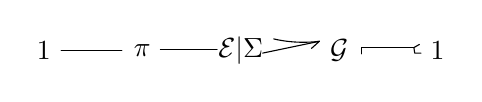
\begin{tikzpicture}[baseline=(extension.base),x=1cm,y=1cm,line cap=round,line join=round]
\node (oneleft) at (0,0) {$1$};
\node (kernel) at (1.25,0) {$\pi$};
\node (extension) at (2.50,0) {$\unsure{\mathcal E|\Sigma}$};
\node (quotient) at (3.75,0) {$\mathcal G$};
\node (oneright) at (5,0) {$1$};
\draw (0.22,0) -- (0.99,0);
\draw (1.48,0.01) -- (2.20,0.01);
\draw (2.78,-0.03) -- (3.50,0.12);
\draw (2.92,0.15) .. controls (3.13,0.10) and (3.35,0.10) .. (3.50,0.12) -- (3.40,0.03);
\draw (4.03,-0.04) -- (4.03,0.04) -- (4.70,0.04);
\draw (4.70,0.04) -- (4.77,0.08);
\draw (4.70,0.04) -- (4.71,-0.03) -- (4.79,-0.03);
\end{tikzpicture}}
\quad\text{et }\mathfrak Z\quad\unsure{\mathcal E|\Sigma}\text{-ens}\ne\varnothing\text{ sur lequel }\pi\text{ opère librement}\right)
\]
$\longleftrightarrow(\Pi,\widetilde\Pi,p,\mathcal G,a)$. On va interpréter la donnée d'un triple $(\inserted{\chi,}\unsure{\tau|\mathcal T},T,\Phi)$, \inserted{$\chi:$} où $\unsure{\tau|\mathcal T}$ est un $\unsure{\mathcal E|\Sigma}$-ens, $T$ un groupe $(\simeq\widehat{\mathbf Z}\;?)$, \inserted{$\chi:\mathcal G\longrightarrow\operatorname{Aut}(T)$ \unsure{$(\simeq\widehat{\mathbf Z}^{*}\unsure{)|?}\;\text{canon.}?)$}} et
\diagram{\begin{tikzcd}[ampersand replacement=\&]
\Phi:\unsure{\tau|\mathcal T} \arrow[r] \& \operatorname{Hom}_{\mathrm{gr}}(T,\pi)
\end{tikzcd}}
compatible avec op. de $\unsure{\mathcal E|\Sigma}$ (opérant
\mspage{18}

\scanpage{21}
\deleted{$\pi$-torseurs. Pour $j\in J$, le $\pi$-torseur correspondant $P_j$ s'envoie dans $\unsure{\tau|\mathcal T}_j=$ fibre de $j\in\unsure{\tau_\pi|\mathcal T_\pi|\tau/\pi|\mathcal T/\pi}$ dans $\unsure{\tau|\mathcal T}$}
\deleted{\deleted{puis}}
\deleted{la fibre de $P_j$ en $t\in\unsure{\tau|\mathcal T}_j$ étant le torseur sous le stabilisateur $\pi_t$ de $t$ dans $\pi$ suivant : on considère}
\diagram{\begin{tikzcd}[ampersand replacement=\&]
\deleted{\Phi(t):T} \arrow[r,phantom,"{\deleted{\longrightarrow}}" description] \& \deleted{\pi}
\end{tikzcd}}
\deleted{alors $\pi_t$ centralise}

Considérons la restriction de l'opération de $\unsure{\mathcal E|\Sigma}$ sur $\unsure{\tau|\mathcal T}$ à $\pi$, d'où un groupoïde $\langle\unsure{\tau|\mathcal T},\pi\rangle$ dont l'ens des objets est $\unsure{\tau|\mathcal T}$, l'ens des $\operatorname{Isom}(t,t')$ étant
\[
\pi_{t\unsure{\mathbin{-}|\to}t'}=\{\lambda\in\pi\mid\lambda t=t'\}.
\]
\deleted{\unsure{Les composantes|La composition}} On a
\[
\pi_0\langle\unsure{\tau|\mathcal T},\pi\rangle=\unsure{\tau|\mathcal T}/\pi\overset{\mathrm{dfn}}{=}J
\]
\[
\pi_1(\unsure{\tau|\mathcal T},t)=\pi_t\quad(\text{stabilisateur de }t\text{ dans }\pi)
\]
et on trouve que $\pi_t$ centralise $\Phi(t)(T)\subset\pi$. On suppose \uline{$T$ commutatif} et $\deleted{\pi_t=\Phi_t(T)}\quad\Phi_t:T\xrightarrow{\sim}\pi_t$ --- \deleted{du} d'autres termes on suppose donné, en plus de $\unsure{\tau|\mathcal T}$ $\unsure{\mathcal E|\Sigma}$-ens de $\pi$-ens,
\mspage{20}

\scanpage{22}
\mspage{11}
un syst. transitif d'iso. entre les $\pi_t$ $(t\in\unsure{\tau|\mathcal T})$, permettant de les identifier tous à un $=T$. Ainsi $\langle\unsure{\tau|\mathcal T},\pi\rangle$ devient un $T$-groupoïde, c.àd. un groupoïde (pas néc. connexe) où les grpes fondamentaux des comp. conn. sont comm. et tous identifiés à $T$.
De plus, $\unsure{\mathcal E|\Sigma}$ opère sur ce $T$-groupoïde (en opérant également sur $T$) via ses opérations sur le système $(\unsure{\tau|\mathcal T},\pi)$ ($\pi$-espace à gauche) en opérant sur $\unsure{\tau|\mathcal T}$ par l'op. donnée et sur $\pi$ via autom int. de $\unsure{\mathcal E|\Sigma}$, enfin sur $T$ via $\mathcal G$ via $\chi\ldots.$

[Si $\unsure{\mathcal E|\Sigma}$ opère sur $\unsure{\tau|\mathcal T}$, restreignant cette op. à $\pi$ on trouve un groupoïde $\langle\unsure{\tau|\mathcal T},\pi\rangle$ sur lequel $\unsure{\mathcal E|\Sigma}$ opère. Supposant ce groupoïde abélien, on a donc une famille de grpes abéliens \inserted{$(T_j)_{j\in J}$} indexée par $J=\unsure{\tau|\mathcal T}/\pi$, sur laquelle opère $\unsure{\mathcal E|\Sigma}$ via $\unsure{\mathcal E|\Sigma}/\pi=\mathcal G$. Ceci dit, on suppose donné une trivialisation de cette famille $(T_j)$ par $T\simeq T_j$, compatible avec op. de
\mspage{21}

\scanpage{23}
$\mathcal G$ --- lequel opère donc sur $T$. Ceci donne naissance automatiquement \unsure{à|:}
\diagram{\begin{tikzcd}[ampersand replacement=\&,column sep=small]
\Phi:\unsure{\tau|\mathcal T}\&\unsure{\longrightarrow|\mathbin{-}}\&\operatorname{Hom}_{\mathrm{gr}}(T,\pi)\qquad\ldots
\end{tikzcd}}

Ceci dit, on a un hom du groupoïde $\langle\unsure{\tau|\mathcal T},\pi\rangle$ dans le groupoïde des rev. universels de $\Pi$, constant sur les objets et de valeur $\widetilde\Pi$ sur ceux-ci, qui envoie donc l'ens des flèches dans $\pi$ --- et qui pour $t,t'\in\unsure{\tau|\mathcal T}$, désignant par
\figure{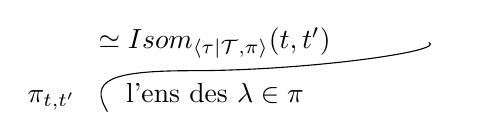
\begin{tikzpicture}[x=1cm,y=1cm]
\node[anchor=base west,inner sep=0pt] at (0,0) {$\pi_{t,t'}$};
\node[anchor=base west,inner sep=0pt] at (1.25,0) {l'ens des $\lambda\in\pi$};
\node[anchor=south west,inner sep=0pt] at (0.90,0.55) {\inserted{$\simeq\operatorname{Isom}_{\langle\unsure{\tau|\mathcal T},\pi\rangle}(t,t')$}};
\draw[thin] (1.02,-0.12) .. controls (0.78,0.28) and (1.05,0.40) .. (2.10,0.40) .. controls (3.55,0.40) and (5.35,0.65) .. (5.10,0.76);
\end{tikzpicture}}
tels que $\lambda t=t'$, est l'inclusion de $\pi_{t,t'}$ dans $\pi$. Ce foncteur
\diagram{\begin{tikzcd}[ampersand replacement=\&]
\langle\unsure{\tau|\mathcal T},\pi\rangle\arrow[r]\&
\begin{gathered}
\text{Cat des}\\
\text{rev. universels}\\
\text{de }\Pi\text{ égaux}\\
\text{\unsure{à|:} }\widetilde\Pi\\
\simeq(\text{un objet}\\
\text{et groupe d'isom---}\\
\pi)
\end{gathered}
\end{tikzcd}}
est évidemment compatible avec op. de $\unsure{\mathcal E|\Sigma}$ sur $\unsure{\Pi|\widetilde\Pi}$ donc sur $\pi\ldots.$
\mspage{22}

\scanpage{24}
\mspage{12}
\figure{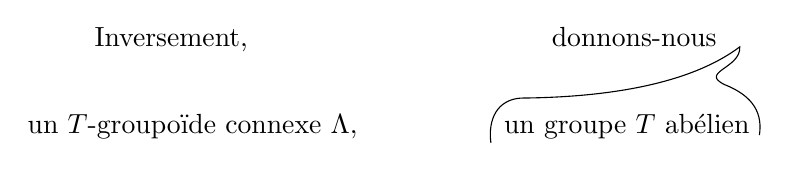
\begin{tikzpicture}[x=1cm,y=1cm]
\node[anchor=base west,inner sep=0pt,text width=7.9cm] at (0,1.10) {Inversement,\hfill donnons-nous};
\node[anchor=base west,inner sep=0pt] at (-0.85,0) {un $T$-groupoïde \deleted{\unsure{connexe}} $\Lambda$,};
\node[anchor=base west,inner sep=0pt] (abelianaddition) at (5.20,0) {\inserted{un groupe $T$ abélien}};
\draw[thin] (5.04,-0.12) .. controls (5.00,0.18) and (5.12,0.43) .. (5.42,0.45)
 .. controls (6.60,0.46) and (7.60,0.65) .. (8.20,1.10)
 .. controls (8.22,0.83) and ([xshift=-0.65cm,yshift=0.78cm]abelianaddition.base east) .. ([xshift=-0.32cm,yshift=0.62cm]abelianaddition.base east)
 .. controls ([xshift=0.06cm,yshift=0.47cm]abelianaddition.base east) and ([xshift=0.16cm,yshift=0.24cm]abelianaddition.base east) .. ([xshift=0.12cm,yshift=-0.02cm]abelianaddition.base east);
\end{tikzpicture}} une opération de $\unsure{\mathcal E|\Sigma}$ sur $(T,\Lambda)$, et un hom de groupoïdes
\diagram{\begin{tikzcd}[ampersand replacement=\&]
\Lambda \arrow[r,"\text{foncteur \uuline{fidèle}}"] \& \begin{gathered}\text{groupoïde \unsure{à|:} un seul objet}\\\text{des rev. universels de}\\\Pi\text{ égaux \unsure{à|:} }\widetilde\Pi\\\text{dont les autom sont }\pi\end{gathered}
\end{tikzcd}}
compatible avec action de $\unsure{\mathcal E|\Sigma}$.
Soit $\unsure{\tau|\mathcal T}=\operatorname{Ob}\Lambda$ [donc $\unsure{\tau|\mathcal T}$ est un $\unsure{\mathcal E|\Sigma}$ ens,] et pour $\forall\,t,t'\in\unsure{\tau|\mathcal T}$, on a un hom \uline{injectif}
\diagram{\begin{tikzcd}[ampersand replacement=\&]
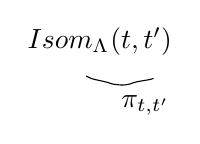
\begin{tikzpicture}[baseline=(isomop.base),x=1cm,y=1cm]
\node[anchor=base west,inner sep=0pt] (isomop) at (0,0) {$\operatorname{Isom}_\Lambda$};
\node[anchor=base west,inner sep=0pt] (isomargs) at (isomop.base east) {$(t,t')$};
\draw[thin] ([xshift=-0.30cm,yshift=-0.35cm]isomop.base east)
 .. controls ([xshift=-0.23cm,yshift=-0.40cm]isomop.base east) and ([xshift=-0.12cm,yshift=-0.40cm]isomop.base east) .. ([yshift=-0.44cm]isomop.base east)
 .. controls ([xshift=0.08cm,yshift=-0.47cm]isomop.base east) and ([xshift=0.20cm,yshift=-0.47cm]isomop.base east) .. ([xshift=0.26cm,yshift=-0.45cm]isomop.base east)
 .. controls ([xshift=-0.45cm,yshift=-0.41cm]isomargs.base east) and ([xshift=-0.32cm,yshift=-0.41cm]isomargs.base east) .. ([xshift=-0.24cm,yshift=-0.38cm]isomargs.base east);
\node[anchor=base west,inner sep=0pt] at ([xshift=0.14cm,yshift=-0.75cm]isomop.base east) {$\pi_{t,t'}$};
\end{tikzpicture} \& \unsure{\hookrightarrow|\lhook\joinrel\relbar} \& \pi
\end{tikzcd}}
compatible avec composition des isom.

On a exprimé la donnée d'un foncteur fidèle d'un groupoïde $\Lambda$ dans $\langle\pi\rangle$ \deleted{Mais \unsure{on}} [il faut se donner une famille de sous groupes $(\pi_t)_{t\in\unsure{\tau|\mathcal T}}$ de $\pi$ et d'ens vides ou bitorseurs sous les $\pi_{t'},\pi_t\ldots$] On va maintenant introduire les op. de
\mspage{23}

\scanpage{25}
$\pi$ sur $\Lambda$, compatibles avec ses op. sur $\pi$ par autom int. Pour ceci, on va exiger
\[
\left\{\begin{gathered}
\forall t\in\unsure{\tau|\mathcal T}=\operatorname{Ob}\Lambda,\quad\text{la famille des}\\
\pi_{t,t'}\subset\pi\quad(t'\in\unsure{\tau|\mathcal T}\text{ variable})\text{ forme une}\\
\text{pseudo-partition de }\pi,\text{ i.e. }\forall\lambda\in\pi,\\
\exists\text{ un unique }t'\text{ tel que }\lambda\in\pi_{t\unsure{,|;}t'}\\
\text{i.e. une unique flèche de }\Lambda\text{ au-dessus}\\
\text{de }\lambda\text{ qui soit d'origine }t.
\end{gathered}\right.
\]
\margin{examinons à part ce condition $\exists!$ de remontage des flèches à origine remontée, pour un morphisme de groupoïdes\ldots}
ce qui donne l'opération de $\pi$ sur $\underset{\unsure{t}}{\unsure{\tau|\mathcal T}=\operatorname{Ob}\Lambda}$, et la façon de reconstituer
\[
\Lambda\simeq\langle\unsure{\tau|\mathcal T},\pi\rangle
\]
et le foncteur $\Lambda\longrightarrow\langle\pi\rangle$. \deleted{\unsure{Dans}} \inserted{On} \deleted{\illegible{1}} suppose de plus que les stabilisateurs $\pi_t$ sont abéliens, d'où une famille de \unsure{grpes|groupes} $(T_j)_{j\in J=\unsure{\tau|\mathcal T}/\pi)}$ et opérations de $\unsure{\mathcal E|\Sigma}$ sur $(T,\Lambda)$, de sorte que $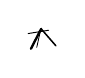
\begin{tikzpicture}[baseline=0pt,x=1em,y=1em,line cap=round,line join=round]
\draw[line width=0.35pt] (-0.10,0.55) -- (0.64,0.67);
\draw[line width=0.30pt] (0.34,0.63) -- (0.21,0.05);
\draw[line width=0.85pt] (0,0) -- (0.37,0.72);
\draw[line width=0.55pt] (0.37,0.72) -- (0.90,0.11);
\end{tikzpicture}\longrightarrow\langle\pi\rangle$ soit compatible avec op. de $\unsure{\mathcal E|\Sigma}$\ldots.

Ce n'est pas bien élucidant --- peut-être est-il plus agréable de
\mspage{24}

\scanpage{26}
\mspage{13}
considérer que \deleted{\unsure{le|que}} $\unsure{\tau|\mathcal T}$
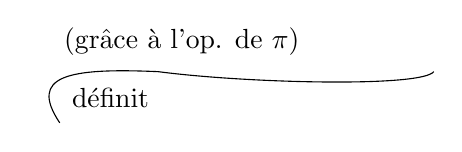
\begin{tikzpicture}[baseline=(main.base),x=1cm,y=1cm]
\node[anchor=base west,inner sep=0pt] (main) at (0,0) {définit};
\node[anchor=south west,inner sep=0pt] at (-0.10,0.65) {\inserted{(grâce à l'op. de $\pi$)}};
\draw[thin] (-0.15,-0.20) .. controls (-0.55,0.40) and (-0.05,0.50) .. (1.10,0.45) .. controls (2.25,0.30) and (4.45,0.25) .. (4.60,0.45);
\end{tikzpicture}
un foncteur
\diagram{\begin{tikzcd}[ampersand replacement=\&,row sep=large,column sep=huge]
\operatorname{Rev}(\Pi)\arrow[r,"F"]\&(\operatorname{Ens})\\
(\pi\text{-}\operatorname{Ens})\arrow[u,"
\begin{tikzpicture}[baseline=-.4ex]\node[rotate=90,inner sep=0pt] {$\approx$};\end{tikzpicture}"',"\begin{gathered}\deleted{\text{via : }\widetilde\Pi}\\E\longmapsto\widetilde\Pi^{\circ}\times_\pi E\end{gathered}"]\arrow[ur,bend right=25,"E\longmapsto\unsure{\tau|\mathcal T}^{\circ}\mathbin{\wedge}_{\pi}E"']
\end{tikzcd}}
[\uline{NB} l'indice $\circ$ indique qu'on a renversé les op. de $\pi$, pour faire opérer $\pi$ à dr)
foncteur commutant aux $\varinjlim$ quelconques. Ceci dit, on veut que $\unsure{\Gamma|F}$ (qui opère sur $\operatorname{Rev}(\Pi)$ via ses opérations sur $\Pi$) soit compatible avec le foncteur $F$, i.e. qu'on ait des isom
\[
F({}^{\gamma}\Pi')\simeq F(\Pi')
\]
$(\Pi'\in\operatorname{Ob}\operatorname{Rev}\Pi)$ fonctoriels en $\Pi'$, et avec transitivité pour $\gamma$ variable. On trouve que cela signifie
\mspage{25}

\scanpage{27}
que l'opération de $\pi$ sur $\unsure{\tau|\mathcal T}$ a été prolongée en une opération de $\unsure{\mathcal E|\Sigma}$ sur $\unsure{\tau|\mathcal T}$. Mais ceci ne donne pas d'interprétation symp. de la $T$- Arrêtons\ldots.
\figure{\begin{tikzpicture}\draw (0,0)--(1.5,0);\end{tikzpicture}}

\textcircled{9} Les schémas et Topos fondamentaux dans la théorie.

\textcircled{A} \deleted{Topos \unsure{Étendus|Étendue}} \inserted{Topos} modulaires 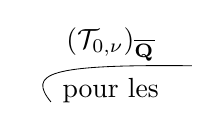
\begin{tikzpicture}[baseline=(words.base)]
\node[anchor=base west,inner sep=0] (words) at (0,0) {pour les};
\node[anchor=base west,inner sep=0] at (0.05,.62) {\inserted{$(\mathcal T_{0,\nu})_{\overline{\mathbf Q}}$}};
\draw[line width=.3pt] (-.14,-.06) .. controls (-.43,.30) and (-.20,.42) .. (1.65,.40);
\end{tikzpicture} courbes de genre $0$ avec $\nu$ points marqués, et famille \deleted{des} modulaire \deleted{\unsure{par}} $\nu$-ponctuée sur $\mathcal T_{0\nu}$\ldots.

Le Topos $(\mathcal T_{0,\nu})_{\mathbf Q}$ pour $\nu=0,1,2$ \uline{n'est} pas un étendu --- car les schémas d'Isom \unsure{d'un|d'une} $X/S$ fibré projectif de rang $1$, avec $\unsure{2|\nu}$ sections marquées (distinctes sur chaque fibre). est lisse de dim rel. $3-\nu\deleted{\unsure{\geq|=|\leq}}>0$ (si $\deleted{\unsure{\nu}}0\leq\nu\leq2$).
\deleted{\unsure{Néanmoins}} \inserted{En fait} ce sont les topos
\figure{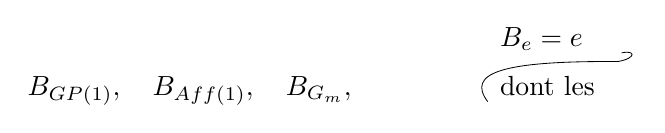
\begin{tikzpicture}[baseline=(list.base)]
\node[anchor=base west,inner sep=0] (list) at (0,0) {$B_{\operatorname{GP}(1)},\quad B_{\operatorname{Aff}(1)},\quad B_{G_m},$};
\node[anchor=base west,inner sep=0] at (6.0,0) {dont les};
\node[anchor=base west,inner sep=0] at (6.0,.62) {$\inserted{B_e=e}$};
\draw[line width=.3pt] (5.85,-.08) .. controls (5.58,.28) and (6.0,.44) .. (7.5,.43) .. controls (7.74,.47) and (7.73,.58) .. (7.55,.54);
\end{tikzpicture}}
\mspage{26}

\scanpage{28}
\mspage{14}
groupes fondamentaux sont \inserted{en apparence} triviaux :
\[
\pi_1(\mathcal T_{0\nu})=0\qquad 0\leq\nu\leq3
\]
Le Topos $\mathcal T_{0,\nu}$ \deleted{est le \inserted{gros} topos fibré} \inserted{$(\nu\geq4)$ correspond au} \deleted{étale de} \inserted{schéma} des syst. de $\nu-3$ points distincts $(x_1,\begin{tikzpicture}[baseline=-.4ex,x=1em,y=1em,line cap=round]
\draw[line width=.35pt] (0,0) -- (.32,.02);
\draw[line width=.30pt] (.54,.02) .. controls (.64,.05) and (.74,-.02) .. (.86,.03);
\end{tikzpicture}\,x_{\nu-3})$ dans
\[
\mathbf P^1-\{0,1,\infty\}=\mathbf E^1\setminus\{0,1\}.
\]
Son groupe fondamental est 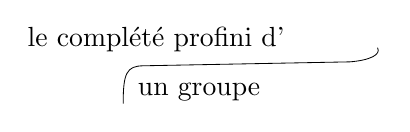
\begin{tikzpicture}[baseline=(base.base)]
\node[anchor=base west,inner sep=0] (base) at (0,0) {un groupe};
\node[anchor=base west,inner sep=0] at (-1.4,.62) {\inserted{le complété profini d'}};
\draw[line width=.3pt] (-.18,-.10) .. controls (-.18,.28) and (-.14,.38) .. (.08,.38) -- (2.7,.43) .. controls (2.95,.45) and (3.1,.52) .. (3.05,.61);
\end{tikzpicture} de tresses $\Pi_{0,\nu}$, lequel (en tant que ``groupe extérieur'') dépend contra-fonctoriellement de $[1,\nu]$ pour les monomorphismes.

Sur $(\mathcal T_{0,\nu})_{\mathbf Q}$ \inserted{du $(\mathcal T_{\unsure{0\nu|0,\nu}})_{\overline{\mathbf Q}}$} on fait opérer $\mathfrak S_\nu$, donc $\mathfrak S_\nu\times\Gamma$ opère sur $\mathcal T_{0,\nu}$,
\figure{
\begin{tikzpicture}[x=1cm,y=1cm]
\fill (0,0) circle (.08);
\fill (.85,.15) circle (.085);
\fill (1.75,.3) ellipse (.21 and .24);
\fill (1.05,-.27) circle (.018);
\fill (1.42,-.34) circle (.035);
\end{tikzpicture}}
\mspage{27}

\scanpage{29}
\mspage{15}
\textcircled{9} \uline{Une conjecture} \uline{arithmético-géométrique}

Soient $g,\nu\geq0$ des entiers. On désigne par $\deleted{\unsure{\mathcal T}}M_{g,\nu}$ le topos modulaire 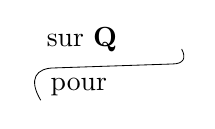
\begin{tikzpicture}[baseline=(base.base)]
\node[anchor=base west,inner sep=0] (base) at (0,0) {pour};
\node[anchor=base west,inner sep=0] at (-0.05,.56) {\inserted{sur $\mathbf Q$}};
\draw[line width=.3pt] (-.12,-.12) .. controls (-.28,.15) and (-.18,.29) .. (.06,.29) -- (1.55,.34) .. controls (1.7,.34) and (1.73,.42) .. (1.67,.53);
\end{tikzpicture} les courbes 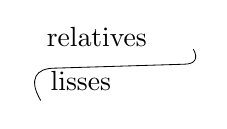
\begin{tikzpicture}[baseline=(base.base)]
\node[anchor=base west,inner sep=0] (base) at (0,0) {lisses};
\node[anchor=base west,inner sep=0] at (-0.05,.56) {\inserted{relatives}};
\draw[line width=.3pt] (-.12,-.12) .. controls (-.28,.15) and (-.18,.29) .. (.06,.29) -- (1.7,.34) .. controls (1.8499999999999999,.34) and (1.88,.42) .. (1.8199999999999998,.53);
\end{tikzpicture} propres relativement connexes de genre $g$, \uline{munies} de \deleted{\unsure{un}} $\nu$-uple de $\nu$ sections disjointes sur chaque fibre

Sauf pour $g=0$, $\nu=0,1,2$ et $g=1$, $\nu=0$, ce topos est associé \unsure{à|:} une étendue algébrique, notion proche = \unsure{schémable}.

On a un hom naturel \deleted{\unsure{extér.}}
\[
\pi_1(\deleted{\unsure{\mathcal T}}M_{g,\nu};\xi)\longrightarrow\operatorname{Autextlac}^{\circ}\bigl(\pi_1(\overline X\setminus\{x_1,\mathbin{-},x_\nu\})\bigr)\tag{1}
\]
où $(X;x_1,\mathbin{-}x_\nu)$ $\longrightarrow$ le pt correspondant 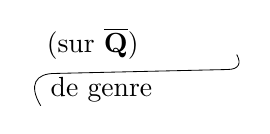
\begin{tikzpicture}[baseline=(base.base)]
\node[anchor=base west,inner sep=0] (base) at (0,0) {de genre};
\node[anchor=base west,inner sep=0] at (-0.05,.56) {\inserted{(sur $\overline{\mathbf Q}$)}};
\draw[line width=.3pt] (-.12,-.12) .. controls (-.28,.15) and (-.18,.29) .. (.06,.29) -- (2.25,.34) .. controls (2.4,.34) and (2.43,.42) .. (2.37,.53);
\end{tikzpicture} $\unsure{g|0}$ avec $\nu$ pts marqués associée à $\xi$ 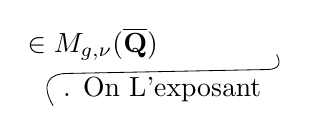
\begin{tikzpicture}[baseline=(base.base)]
\node[anchor=base west,inner sep=0] (base) at (0,0) {. \deleted{On} L'exposant};
\node[anchor=base west,inner sep=0] at (-0.45,.56) {\inserted{$\in M_{g,\nu}(\overline{\mathbf Q})$}};
\draw[line width=.3pt] (-.12,-.12) .. controls (-.28,.15) and (-.18,.29) .. (.06,.29) -- (2.6,.34) .. controls (2.75,.34) and (2.7800000000000002,.42) .. (2.72,.53);
\end{tikzpicture} $\circ$ marque le fait qu'on prend les autom de $\pi_1$ qui n'échangent pas entre eux les classes de lacets associés aux $x_i$\unsure{--|.}
\margin{il faut peut-être être plus strict, et exiger la commutation : des opérations : définies de $\mathfrak S_\nu$ sur le $\pi_1$ ?? Il faut regarder surtout le cas $g=0,\nu=3$....}

Notons qu'on a aussi
\[
\pi_1(\overline M_{g,\nu};\xi)\longrightarrow\operatorname{Autextlac}^{\circ\circ}\bigl(\pi_1(X\setminus\{x_1,\mathbin{-}x_\nu\})\bigr)\tag{2}
\]
où le double $\circ$ indique qu'on prend des autom \inserted{\uline{stricts}} compatibles avec la structure : \unsure{locale|lacets}, \unsure{(i.e.|i.e.} induisant l'identité sur $T=\operatorname{Tate}(\overline{\mathbf Q})$\ldots
\margin{Aut. \unsure{orientés}}
\[
\pi_1(M_{g,\nu}^{an};\xi)\longrightarrow
\mathrm{Aut}\underbrace{\mathrm{extlac}^{\circ\circ}\pi_1(X^{an}\setminus\{}_{\overset{\unsure{\deleted{
\begin{tikzpicture}[baseline=0pt,x=.45em,y=.4em,line width=.45pt,line cap=round,line join=round]\draw (0,.12) .. controls (.08,.18) and (.25,.56) .. (.27,.91) -- (.21,.19) .. controls (.19,.02) and (.33,.11) .. (.39,.34) -- (.66,1.05) .. controls (.62,.70) and (.58,.16) .. (.64,-.08) .. controls (.66,-.14) and (.76,.18) .. (.80,.26) -- (1.28,.20) -- (1.30,.10);\end{tikzpicture}}}}{=}\mathcal T_{g,\nu}\ (\text{Teichmüller})}x_1,\mathbin{-}x_\nu\})\tag{2 bis}
\]
dont on sait (théorie top.) que c'est un
\mspage{28}

\scanpage{30}
\uline{isomorphisme}, et dont (2) se déduit en passant au profini. On a ainsi un 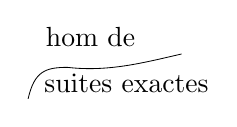
\begin{tikzpicture}[baseline=(base.base)]
\node[anchor=base west,inner sep=0] (base) at (0,0) {suites exactes};
\node[anchor=base west,inner sep=0] at (.02,.58) {\inserted{hom de}};
\draw[line width=.3pt] (-.20,-.08) .. controls (-.12,.27) and (.02,.32) .. (.30,.32) .. controls (.82,.26) and (1.27,.38) .. (1.75,.49);
\end{tikzpicture}
\margin{sauf si $g=0,\nu=0,1,2$\quad\figure{\begin{tikzpicture}\node[draw,ellipse] {$g=1,\nu=0$};\end{tikzpicture}}?}
\diagram{(4)\quad\begin{tikzcd}[ampersand replacement=\&,column sep=small,row sep=large]
1 \arrow[r,dash] \& \pi_1(\overline M_{g,\nu};\unsure{\xi|j}) \arrow[r,dash] \arrow[d,"\tikz[baseline=-.5ex]{\node[rotate=90,inner sep=0pt] {$\approx$};}"',"\deleted{\unsure{\mathcal T_{g\nu}^{\wedge}}}"] \& \pi_1(M_{g,\nu};\unsure{\xi|j}) \arrow[r] \arrow[d] \& \Gamma \arrow[r,dash] \arrow[d,bend left=20] \& 1\\
1 \arrow[r] \& \mathcal T_{g,\nu}^{\wedge} \arrow[r] \& \operatorname{Autextlac}^{\circ}(\pi_1(X_{\unsure{\xi|j}}\setminus\{x_1,-x_\nu)) \arrow[r] \& \operatorname{Out}\unsure{T} \arrow[d,phantom,"\unsure{\vert|\downarrow}" description]\\
\&\&\&1
\end{tikzcd}}
\unsure{admettons} que $\mathcal T_{g,\nu}^{\wedge}\unsure{\to|\text{est}}$
\unsure{invariant|injective} dans $\operatorname{Autextlac}^{\circ}(\ ?\ )$.
\margin{Version corrigée éventuelle : $\pi_1(M_{g,\nu};\unsure{\xi|j})\simeq$ Normalisateur de $\mathcal T_{g,\nu}^{\wedge}$ dans $\operatorname{Autextlac}^{\circ}(\pi_1(X_{\unsure{\xi|j}}\setminus\{x_1-x_\nu\unsure{\})|\}))}$ induisant des \unsure{autom} de $\mathcal T_{g,\nu}^{\wedge}$ commutant à $\mathfrak S_\nu$ et préservant une structure
\figure{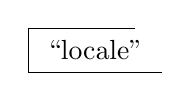
\begin{tikzpicture}
\node[inner sep=1pt] (loc) at (0,0) {``locale''};
\draw (-.85,.28)--(-.85,-.28)--(.85,-.28);
\draw (-.85,.28)--(.5,.28);
\end{tikzpicture}}
éventuelle\ldots $*$
\figure{\begin{tikzpicture}\draw (0,0)--(3.7,0);\end{tikzpicture}}}

On \deleted{\unsure{a}} aimerait que la flèche (1) (la flèche verticale centrale de (5)) soit un \uline{iso}. Cela donnerait une caractérisation de $\Gamma$ comme
\[
\operatorname{Autextlac}^{\circ}\left(\pi_1\underbrace{(X^{an}\setminus\{x_1,-x_\nu\})^{\wedge}}_{\substack{\text{groupe standard}\\\text{bien connu}}}\right)/\mathcal T_{g,\nu}^{\wedge}
\]
\margin{Pour $(g,\nu)$ sauf $g=0,\nu=0,1,2$\quad $g=1,\nu=0$ (cas où $\pi_1(X_{\unsure{\overline{\mathbf Q}|\mathbf Q}}\setminus S_\nu)$ \unsure{est un gr|est un groupe} abélien).
\figure{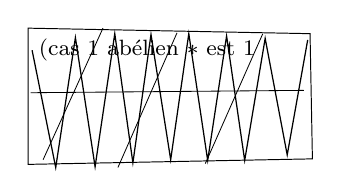
\begin{tikzpicture}
\node[anchor=north west,align=left,text width=3.4cm,font=\footnotesize,inner sep=0] at (0,.85) {\deleted{\unsure{(cas} \illegible{1} \unsure{abélien} $*$ \unsure{est} \illegible{1}}};
\draw[line width=.35pt] (-.13,-.75)--(-.13,.98)--(3.45,.91)--(3.48,-.68)--cycle;
\draw[line width=.45pt] (-.08,.70)--(.22,-.79)--(.47,.86)--(.72,-.78)--(.97,.91)--(1.20,-.73)--(1.43,.90)--(1.68,-.69)--(1.91,.91)--(2.15,-.70)--(2.39,.88)--(2.62,-.70)--(2.88,.85)--(3.16,-.63)--(3.42,.83);
\draw[line width=.3pt] (.06,-.69)--(.82,.98) (1.01,-.79)--(1.76,.92) (2.12,-.74)--(2.85,.91) (-.10,.16)--(3.37,.19);
\end{tikzpicture}}}
\margin{Pour le cas $g=0,\nu=3$, il convient aussi d'être prudent et d'exiger des conditions de commutations avec \unsure{op|op.} ext. de $\mathfrak S_3$\ldots}

\uline{Ex} Pour $g=0,\nu=3$ celà donnerait l'expression déjà envisagée de $\Gamma$ comme
\[
\operatorname{Autextlac}^{\circ}(\pi_1(\mathbf P^1\setminus\{0,1,\infty\}).
\]
\mspage{29}

\scanpage{31}
\mspage{16}
Si on considère le quotient \inserted{$N_{g,\nu}$} de $M_{g,\nu}$ par $\mathfrak S_\nu$ (de sorte que $M_{g,\nu}$ est un rev. de groupe $\mathfrak S_\nu$ de $N_{g,\nu}$) \unsure{on a|\ldots}
\diagram{\begin{tikzcd}[ampersand replacement=\&,column sep=small,row sep=small]
(5)\quad1 \arrow[r] \& \pi_1(\overline M_{g,\nu}) \arrow[r] \&
\pi_1(N_{g,\nu},\xi) \arrow[rr] \arrow[dr,phantom,"="] \arrow[dd,phantom,"\Vert"] \& \&
\mathfrak S_\nu\times\Gamma \arrow[r] \& 1\\
\& \& \& \pi_1(\overline N_{g,\nu},\Gamma;\unsure{\xi|j}) \arrow[d,phantom,"\Vert"]\\
\& \& \pi_1(M_{g,\nu},\mathfrak S_\nu,\xi) \arrow[r,phantom,"="] \&
\pi_1(\overline M_{g,\nu},\mathfrak S_\nu\times\Gamma)
\end{tikzcd}}
structure d'extension un peu plus riche que la première ligne de (4). La conjecture \unsure{faite|fait} équivaut \unsure{à|:} la suivante :
\[
\pi_1(N_{\unsure{g\nu|g,\nu}};\xi)\xrightarrow{\sim}\operatorname{Autextlac}\bigl(\pi_1(X_{\unsure{\xi|j}}\setminus\{x_1,\mathbin{-}x_\nu\})\bigr)
\]
ou encore
\[
\Gamma\simeq\operatorname{Autextlac}\bigl(\pi_1(X_{\unsure{\xi|j}}\setminus\{x_1,\mathbin{-}x_\nu\})\bigr)/\widetilde{\mathcal T}_{g,\nu}^{\wedge}
\]
où
\[
\widetilde{\mathcal T}_{g\nu}\simeq\operatorname{Autextlac}^{+}\bigl(\pi_1(X_{\unsure{\xi|j}}^{an}\setminus\{x_1,\mathbin{-}x_\nu\}).
\]

$*$ NB Il faudrait déterminer le groupe des automorphismes 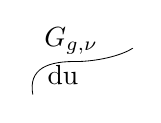
\begin{tikzpicture}[baseline=(base.base)]
\node[anchor=base west,inner sep=0] (base) at (0,0) {du};
\node[anchor=base west,inner sep=0] at (-.04,.48) {\inserted{$G_{g,\nu}$}};
\draw[line width=.3pt] (-.18,-.13) .. controls (-.24,.20) and (.01,.30) .. (.40,.29) .. controls (.70,.30) and (.97,.38) .. (1.09,.46);
\end{tikzpicture} topos modulaire géom $\overline M_{g,\nu}$ \deleted{\unsure{est}} ($G_{g,\nu}=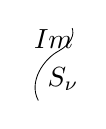
\begin{tikzpicture}[baseline=(base.base)]
\node[anchor=base west,inner sep=0] (base) at (0,0) {$\mathfrak S_\nu$};
\node[anchor=base west,inner sep=0] at (-.17,.48) {$\inserted{\operatorname{Im}}$};
\draw[line width=.3pt] (-.11,-.18) .. controls (-.24,.06) and (-.04,.35) .. (.15,.45) .. controls (.31,.54) and (.35,.66) .. (.32,.74);
\end{tikzpicture}$ ? \unsure{\deleted{)}|\}} Sans doute $\mathfrak S_\nu$ opère fidèlement sauf $g=0,\nu\leq4$\textendash\,\textemdash)

\uline{Question}
\[
\Gamma\longrightarrow\operatorname{Autext}\,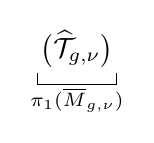
\begin{tikzpicture}[baseline=(arg.base)]
\node[inner sep=1pt] (arg) {$\bigl(\widehat{\mathcal T}_{g,\nu}\bigr)$};
\draw ([yshift=-1pt]arg.south west) -- ([yshift=-5pt]arg.south west) --
      ([yshift=-5pt]arg.south east) -- ([yshift=-1pt]arg.south east);
\node[anchor=north,inner sep=1pt] at ([yshift=-5pt]arg.south)
      {$\scriptstyle\pi_1(\overline M_{g,\nu})$};
\end{tikzpicture}
\quad\left\{\begin{array}{l}\text{injectif ?}\\\text{bijectif}\end{array}\right.
\]
\margin{(Sans doute il faut condition \unsure{sur le} \illegible{1}, cf NB.}
\mspage{30}

\scanpage{33}
\margin{\begin{tabular}{c}
IBM\\IBM\\IBM\\IBM\\IBM\\IBM\\IBM\\IBM\\IBM\\IBM\\IBM\\IBM\\IBM\\IBM\\IBM\\IBM\\IBM\\IBM\\IBM\\IBM\\IBM\\IBM\\IBM\\IBM\\IBM\\IBM\\IBM\\IBM\\IBM\\IBM\\IBM
\end{tabular}}
\diagram{\begin{tikzcd}[ampersand replacement=\&,column sep=small,row sep=small]
1 \arrow[dr,dash] \& 1 \arrow[dr,dash]\\
1 \arrow[r] \& \pi_1(\overline X_{\unsure{\xi|g}}\setminus S_\nu) \arrow[r] \arrow[dr] \& \pi_1(\overline X_{\unsure{j|\xi}}S_\nu) \arrow[r] \arrow[dr] \& 1 \arrow[dr]\\
\&1 \arrow[r] \& \pi_1(\overline M_{g,\nu+1}) \arrow[r] \arrow[dr] \& \pi_1(M_{g,\nu+1}) \arrow[r] \arrow[dr] \& \Gamma \arrow[r,phantom,"{\unsure{\longleftarrow|\longrightarrow}}" description] \arrow[dr] \&1\\
\&\&1 \arrow[r] \& \pi_1(\overline M_{g,\nu}) \arrow[r] \arrow[dr] \& \pi_1(M_{g,\nu}) \arrow[r] \arrow[dr,Rightarrow] \& \Gamma \arrow[r,phantom,"{\unsure{\longrightarrow|\relbar}}" description] \arrow[dr,Rightarrow] \&1\\
\&\&\&\&1\&1\&1
\end{tikzcd}}
\diagram{\begin{tikzcd}[ampersand replacement=\&,column sep=small,row sep=small]
1 \arrow[dr,dash] \&1 \arrow[dr]\\
1 \arrow[r] \& \begin{gathered}\widehat{\pi}_{g,\nu}\\[-.25ex]\makebox[0pt][c]{\hspace{-3.4em}$\deleted{\unsure{1}\mathbin{-}\unsure{\pi_{g,\nu}(X)|\pi_1(X)}}$}\end{gathered} \arrow[r,"\sim"] \arrow[dr] \& \widehat{\pi}_{g,\nu} \arrow[r] \arrow[dr] \&1 \arrow[dr,dash]\\
\&1 \arrow[r] \& \widehat{\mathcal T}_{g,\nu+1} \arrow[r] \arrow[dr] \& \operatorname{Autlac}^{\circ}(\widehat{\pi}_{g,\nu})^{!} \arrow[r] \arrow[dr] \& \Gamma \arrow[r] \arrow[dr,phantom,"{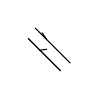
\begin{tikzpicture}[x=.65cm,y=.65cm,line cap=round,baseline=-.15cm]\draw (0,.58)--(.68,-.10);\draw (-.14,.38)--(.49,-.25);\draw (.22,.36)--(.13,.49);\draw (.09,.15)--(.22,.17);\end{tikzpicture}}" description] \&1\&\hspace{1.7em}\Sigma_{\nu+1}\\
\&\&1 \arrow[r] \& \widehat{\mathcal T}_{g,\nu} \arrow[r] \arrow[dr] \& \operatorname{Autextlac}^{\circ}(\widehat{\pi}_{g,\nu})^{!} \arrow[r,"{\text{traces}}"'] \arrow[dr] \&\Gamma \arrow[r,dash] \&1\&\hspace{1.7em}\Sigma_\nu\\
\&\&\&\&1\&1
\end{tikzcd}}
\[
\begin{gathered}
M'_{g,\nu}(K)\ni\xi\\
\mathcal T'_{g,\nu}\ni G_\xi
\end{gathered}
\]
\diagram{\ensuremath{\begin{array}{@{}r@{\;}c@{\qquad\qquad}c@{}}
\deleted{\unsure{\Gamma_g|\Sigma_g}}&&\\
&\widehat\Sigma_{g,\nu}^{\sim}&\Sigma_{g,\nu}\\
&\Vert&\\
&\overline\Sigma_{g,\nu}&
\end{array}}}
\margin{\begin{tabular}{c}6\\5\\4\\3\\2\\1\\0\end{tabular}}
\margin{2975 -- 132}
\mspage{32}

\scanpage{34}
\diagram{\ensuremath{\begin{array}{rrrr}
************&0.0000&&\\
************&**********&&\\
************&**********&&\\
75.000&&&\\
0.0307&20.4842&0.9297&\\
0.0309&21.3976&0.9048&\\
0.0310&22.3325&0.8763&\\
0.0311&23.2828&0.8443&\\
0.0313&24.2418&0.8090&\\
0.0314&25.2032&0.7705&\\
0.0315&26.1611&0.7289&\\
0.0317&27.1095&0.6845&\\
0.0318&28.0431&0.6374&\\
0.0319&28.9568&0.5878&\\
0.0321&29.8459&0.5358&\\
0.0322&30.7065&0.4817&\\
0.0323&31.5349&0.4258&\\
0.0325&32.3279&0.3681&\\
0.0326&33.0829&0.3090&\\
0.0327&33.7976&0.2487&\\
0.0329&34.4703&0.1874&\\
0.0330&35.0994&0.1253&\\
0.0331&35.6839&0.0628&\\
0.0333&36.2229&0.0000&\\
0.0334&36.7160&-0.0627&\\
0.0335&37.1629&-0.1252&\\
0.0337&37.5634&-0.1873&\\
0.0338&37.9177&-0.2486&\\
0.0339&38.2260&-0.3089&\\
0.0341&38.4885&-0.3680&\\
0.0342&38.7058&-0.4257&\\
0.0343&38.8783&-0.4816&\\
0.0345&39.0067&-0.5357&\\
0.0346&39.0916&-0.5877&\\
0.0347&39.1337\smash{\raisebox{-.5\baselineskip}{$\inserted{\Big)\,\text{max}}$}}&-0.6373&\\
0.0349&39.1337&-0.6844&\\
0.0350&39.0925&-0.7289&\\
0.0351&39.0108&-0.7704&\\
0.0353&38.8894&-0.8089&\\
0.0354&38.7293&-0.8442&\\
0.0355&38.5313&-0.8762&\\
0.0357&38.2964&-0.9047&\\
0.0358&38.0256&-0.9297&\\
0.0359&37.7197&-0.9510&\\
0.0361&37.3799&-0.9685&\\
0.0362&37.0072&-0.9822&\\
0.0363&36.6027&-0.9920&\\
0.0365&36.1675&-0.9980&\\
0.0366&35.7027&-1.0000&\\
0.0367&35.2095&-0.9980&\\
0.0369&34.6893&-0.9921&\\
0.0370&34.1432&-0.9823&\\
0.0371&33.5725&-0.9686&\\
0.0373&32.9788&-0.9510&\\
0.0374&32.3633&-0.9298&\\
0.0375&31.7275&-0.9048&\\
0.0377&31.0730&-0.8763&\\
0.0378&30.4013&-0.8444&\\
0.0379&29.7141&-0.8091&\\
0.0381&29.0130&-0.7706&\\
0.0382&28.2999&-0.7290&\\
0.0383&27.5764&-0.6846&\\
0.0385&26.8445&-0.6375&\\
0.0386&26.1062&-0.5879&\\
0.0387&25.3634&-0.5359&\\
0.0389&24.6183&-0.4818&
\end{array}}}
\[
\begin{aligned}
\Delta U&=26.3878\ \unsure{\mathrm{m/s}|\mathrm{m/o}}\\
U_m&=25.939\ \unsure{\mathrm{m/s}|\mathrm{m/o}}
\end{aligned}
\]
\diagram{\ensuremath{\begin{array}{r}
39.1337\\12.7459\\\hline26.3878
\end{array}}}
\diagram{\ensuremath{\begin{array}{r}
12.7459\\13.1939\\\hline25.9398
\end{array}}}
\mspage{33}

\cotefile{145}

\scanpage{2}
\deleted{bien \unsure{distinguer|déterminé} $\bar D_{J,\alpha}$ de $\bar D_J$, cf. \unsure{9}}
\deleted{\diagram{\begin{tikzcd}
\bar U_{J',\alpha'} \arrow[r] \arrow[d] & \bar U_{J,\alpha} \arrow[r] \arrow[d] & \bar U \arrow[d] \\
U_{J',\alpha'} \arrow[r] & U_{J,\alpha} \arrow[r] & U
\end{tikzcd}}}

\diagram{\begin{tikzcd}[column sep=small]
D=U(\mathbb C)^{\sim} \arrow[rr] \arrow[dr,"\pi"'] && \widetilde U(\mathbb C)\deleted{\unsure{\ne U|=U}} \arrow[dl,"\hat\pi"] \\
& U(\mathbb C) &
\end{tikzcd}}
\[ \pi\subset G \]
\[
H_{\deleted{\unsure{u}}}=\bigl\{u\in G\mid \exists
\underset{\substack{\text{\unsure{ss=gr.|ss-gr.}}\\\text{d'indice fini}}}{\begin{gathered}\pi'\subset\pi\\[-.8ex]
\begin{tikzpicture}[x=1cm,y=1cm,baseline=0pt]\draw (0,.09) .. controls (-.04,-.01) and (-.01,-.05) .. (.10,-.05)--(1.25,-.05) .. controls (1.38,-.05) and (1.38,.03) .. (1.30,.09);\end{tikzpicture}\end{gathered}},\quad
\underset{\text{id.}}{\begin{gathered}\pi''\subset\pi\\[-.8ex]
\begin{tikzpicture}[x=1cm,y=1cm,baseline=0pt]\draw (0,.09) .. controls (-.04,-.01) and (-.01,-.05) .. (.10,-.05)--(1.25,-.05) .. controls (1.38,-.05) and (1.38,.03) .. (1.30,.09);\end{tikzpicture}\end{gathered}},
\quad\text{iso }v:D/\pi'\simeq D/\pi'',\quad\text{avec}
\]
\diagram{\begin{tikzcd}
D \arrow[r,"u"] \arrow[d,"p'"'] & D \arrow[d,"p''"] & \text{commutatif} \\
D/\pi' \arrow[r,"\substack{v\\\sim}"] & D/\pi'' &
\end{tikzcd}}

\uline{NB} On aura, pour $u,\pi',\pi'',v$ comme dessus un iso
\figure{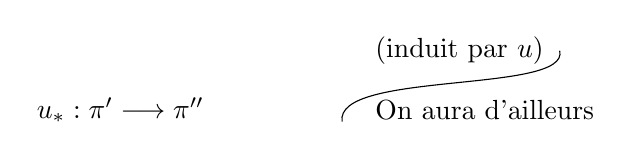
\begin{tikzpicture}
\node[anchor=west] (map) at (0,0) {$u_*:\pi'\longrightarrow\pi''$};
\node[anchor=west] (ins) at (4.3,.75) {\inserted{(induit par $u$)}};
\draw ([xshift=.08cm]ins.east) .. controls (6.9,.2) and (3.9,.5) .. (4,-.15);
\node[anchor=west] at (4.3,0) {On aura d'ailleurs};
\end{tikzpicture}}
$\pi'$ et $\pi''$ de $=$ indice dans $\pi$.
\margin{$u$ est déterminé par $v_*$}

\uline{NB} $v$ est connu quand on connaît $v_*$ (\uline{ces conditions}), et quand $v$ est connu, $u$ est connu \deleted{\unsure{aux}} mod multiplication \uline{\unsure{à|:} gauche} par un $\gamma\unsure{\in|+}\pi''$.

\margin{\diagram{\begin{tikzcd}[column sep=small]
& \pi & \\
\pi' \arrow[ur,phantom,"\tikz[baseline=-.5ex]{\node[rotate=-35,inner sep=0pt] {$\cup$};}" description] \arrow[rr,phantom,"\simeq" description] && \pi'' \arrow[ul,phantom,"\tikz[baseline=-.5ex]{\node[rotate=15,inner sep=0pt] {$\cup$};}" description]
\end{tikzcd}}
\[\pi_i'\simeq\pi_i''\]}
\margin{\[
p''u=vp'
\]
\[\deleted{p''u\gamma=}\]
\[p''(\gamma u)=(p''\gamma)u=p''u=vp')\]
\[\deleted{\pi\subset H}\]}

$H$ est un groupe $\supset\pi$, et $H/\pi$ (classes \unsure{à|:} droite) s'identifie à un sous-ens de \unsure{l'ens|l'un} des ``germes'' \uline{d'isom} \deleted{\unsure{des}} $H$-groupes d'indice \unsure{finis|fini} de $\pi$ de $=$ indice

$H_n=$ sous-ens de $H$ formé des $u$ pour lesquels on peut prendre $\pi',\pi''$ d'indice $n$.

$H_n$ est un \uline{ss-groupe}, et $\pi$ d'indice
\mspage{1}
